\documentclass[a4paper,12pt,openany,oneside]{article}
\usepackage{geometry}
 \geometry{
 	a4paper,
 	left=25mm,
 	top=30mm,
 	bottom=40mm,
 	right=25mm
 }
\usepackage{lmodern}

% Packages AMS
\usepackage{amsmath}
\usepackage{mathtools}
\usepackage{amsfonts}
\usepackage{listings}
\usepackage{amssymb}
\usepackage{amsthm}
\usepackage{url}
% Simboli matematici aggiuntivi
\usepackage{stmaryrd}
\usepackage{verbatim}
% Per creare l'indice
\usepackage{index}
% Per spazi dopo le macro
\usepackage{xspace}
% Importazioni e manipolazione di grafica
\usepackage{graphicx}
% Per \begin{comment} ... \end{comment}
\usepackage{comment}
% Per la spaziatura tra linee
\usepackage{setspace}
% Per una migliore resa tipografica con pdflatex
\usepackage{microtype}

\usepackage{enumitem}

\usepackage{booktabs}
\usepackage{tabularx}
\usepackage{float}
\usepackage[final]{pdfpages}
\usepackage{caption}
\usepackage[hidelinks]{hyperref}
\usepackage{float}
\usepackage{helvet}
\usepackage{subcaption}

% Per i disegni
\usepackage{tikz}
\usetikzlibrary{calc,patterns,angles,quotes}
\usepackage{tkz-euclide}
\usetkzobj{all}
\usetikzlibrary{arrows}

% Per font piccolo caption
\usepackage[font=footnotesize]{caption}

\usepackage{nameref}

\usepackage[T1]{fontenc}
\usepackage[utf8]{inputenc}
\usepackage{babel}
\usepackage{numprint}
\npthousandsep{\,}

% Per quote belli 
\newcommand{\quotes}[1]{``#1''}

\usepackage[style=verbose]{biblatex}

\usepackage{filecontents}% to embed the file `myreferences.bib` in your `.tex` file

\begin{filecontents}{myreferences.bib}
@inproceedings{nagmoti2010ranking,
  title={Ranking approaches for microblog search},
  author={Nagmoti, Rinkesh and Teredesai, Ankur and De Cock, Martine},
  booktitle={Proceedings of the 2010 IEEE/WIC/ACM International Conference on Web Intelligence and Intelligent Agent Technology-Volume 01},
  pages={153--157},
  year={2010},
  organization={IEEE Computer Society}
}
\end{filecontents}
\addbibresource{myreferences.bib}

\onehalfspacing

\title{Personalized Search Engine for Microblog Content\\ \large{Information Retrieval Project Report}}
\date{January 2019}
\author{\normalsize Matteo Costantini \\ \normalsize 795125 \and \normalsize Dario Gerosa \\ \normalsize 793636 \and \normalsize Michele Perrotta \\ \normalsize 795152}

\makeindex

\begin{document}
\selectfont
\maketitle

\section{Introduction}
The goal of the project is to build a Search Engine for tweets crawled from Twitter. The solution must also offer personalised results with respect to a query using document-based personalization approach.
The user have the option to select a topic and submit a query which will then customise the results based on the documents provided by the user to the system.

The proposed solution implements a Search Engine based on Lucene with re-ranking of the results to take into account the nature of the documents and the platform from which they come from (e.g. retweets and author's followers). The personalization is performed using a \textit{bag-of-words} model with query expansion. All those functionalities are exposed via a Spring web service and a webapp written in Python with Flask allow to submit a query to the Search Engine and display the results.

The crawler used to gather tweets to be indexed by the Search Engine is written in Python using a wrapper of the officials \textit{Twitter's APIs} and uses a \textit{PostgreSQL} database to store the raw documents before pre-processing and indexing.
\begin{figure}[t]
    \centering
    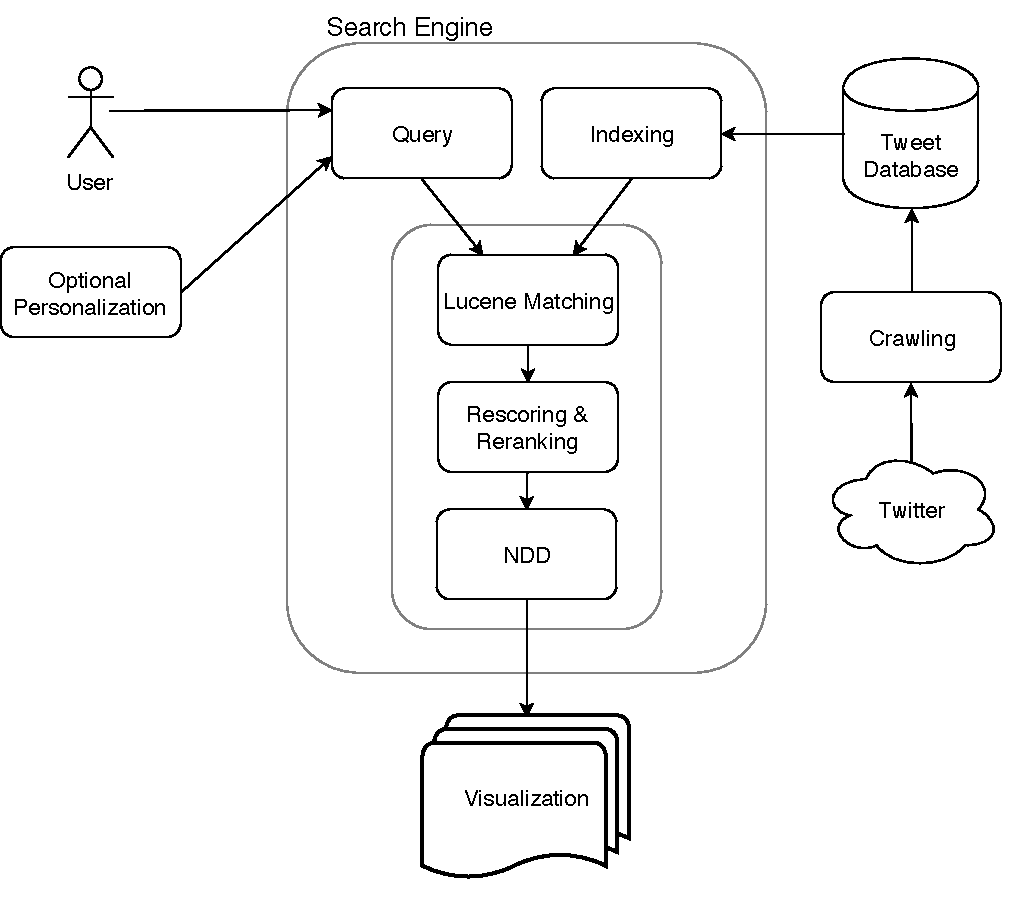
\includegraphics[width=0.8\textwidth]{search_engine.pdf}
    \caption{Overview of the system}
    \label{fig:search_engine}
\end{figure}

\section{Crawling Process}

The first step consisted in the implementation of a crawler in order to retrieve tweets from Twitter. For the assigned task we decided to opt for a focused crawling approach. A list of user has been selected for each topic of interest and for each user the crawler retrieved at most \numprint{3200} tweets (which is the upper limit imposed by Twitter APIs). Each list has been chosen using the Twitter's \textit{lists} feature to find relevant profiles which tweets about the given topic.
The crawler has been implemented in Python using the \verb|tweepy| package which wraps Twitter's official APIs using a PostgreSQL database to persist the data and the \verb|multiprocessing| module to speed up the crawling process. The first phase consists in retrieving all the information regarding the selected users and storing them in the database. The second step is where the actual crawling of the tweets takes place. 
The crawler has been designed as a concurrent system: each process selects a new user to be processed from a shared queue containing all the users whose tweets need to be saved, then retrieves all the available tweets and after a basic pre-processing stores them in the database.

\begin{figure}[!h]
    \centering
    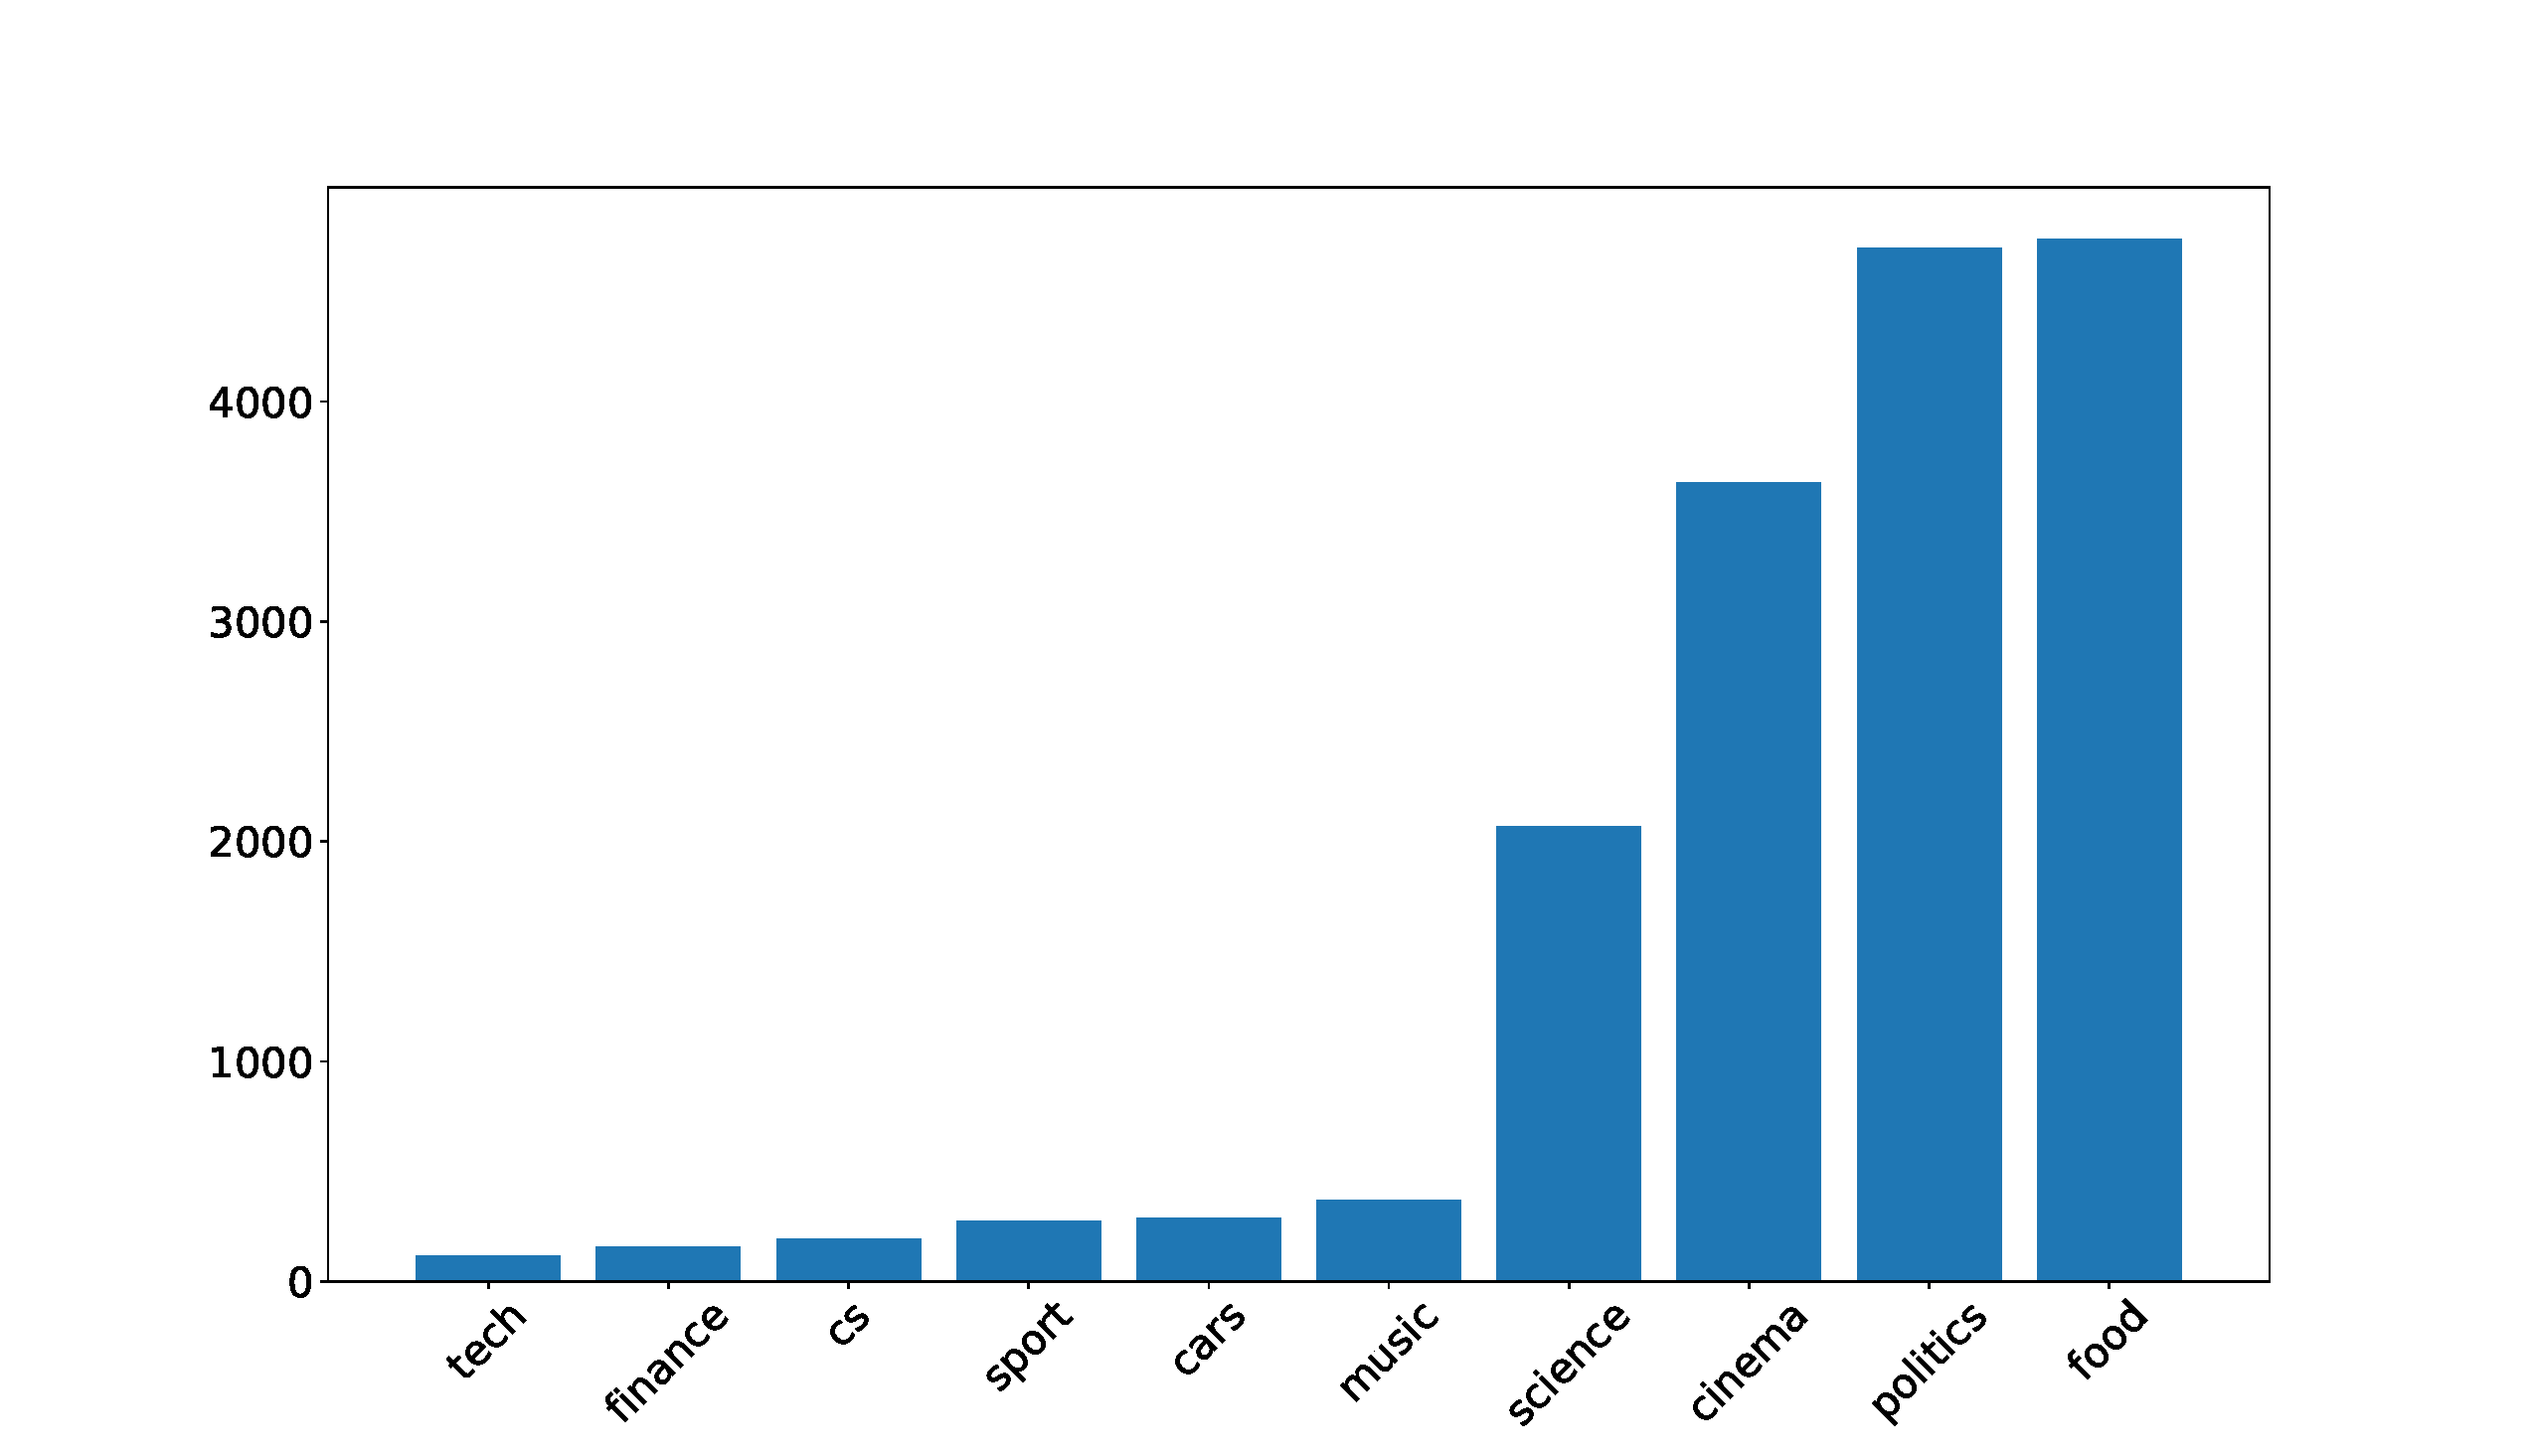
\includegraphics[width=1\textwidth]{topics.eps}
    \caption{Number of users for each topic}
    \label{fig:users-distribution}
\end{figure}


\subsection{Dataset}

In total \numprint{35699286} tweets have been crawled from \numprint{16185} different twitter users after discarding all the tweets in a language different than english (based on the \verb|lang| field in the JSON). The crawler stored, for each user, its followers, the topic to which the user belongs and the raw JSON returned by Twitter's APIs. In the same way, for each tweet its author and the corresponding raw JSON has been stored.

In figure \ref{fig:users-distribution} the distribution of users for each topic taken into account.
It can be seen that the number of users is not uniformly distributed among topics and four of them have significantly more users. We decided not to use the same number of users in each topic since in the real world - not necessarily for the same categories used in this project - we expect that there are topics more discussed than others.

\begin{table}[ht]
	\scriptsize
	\centering	
	\begin{tabularx}{0.24\textwidth}{r r}		
		%\toprule		
		\textbf{Percentile} & \textbf{Follower}\\				
		\midrule				
			5    & 226                  \\
			10   & 391                  \\
			20   & 746                  \\
			30   & \numprint{1210}      \\
			40   & \numprint{1879}      \\
			50   & \numprint{2954}      \\
			60   & \numprint{4625}      \\
			70   & \numprint{7851}      \\
			80   & \numprint{14563}     \\
			90   & \numprint{39785}     \\
			95   & \numprint{105922}    \\
			97   & \numprint{231844}    \\
			99   & \numprint{1262254}   \\
			99.5 & \numprint{3120360}   \\
			100  & \numprint{104683236} \\
		\vspace{5pt}
		%\bottomrule \\
	\end{tabularx}
	\captionof{table}{} 
	\label{tab:percentile_follower} 	
\end{table}
\noindent
In Table \ref{tab:percentile_follower} instead are reported the percentiles of the followers. It can be seen that almost 30\% has less than \numprint{1000} followers and about 5\% of the most followed users have more than 100 000 followers with the majority of the others having between \numprint{10000} and \numprint{40000} followers.

\section{Indexing Process}
To index the documents a custom Lucene Analyzer has been adopted.
The implemented custom Analyzer is based on the \textit{Lucene Classic Analyzer} in addition of some \textit{TokenFilter}.

\begin{enumerate}
    \item \textbf{Addresses filter}: discards URLs and email addresses. Tweets contain usually shortened urls which doesn not carry any kind of information.
    \item \textbf{Classic Tokenizer}: produces tokens using spaces and 
    punctuation as splitting point and discards them.
    Unlike the Standard Tokenizer, the Classic Tokenizer preserves URLs, email addresses and strings with alphabetic characters and numbers separated with hyphens. Special characters such as \verb|( ) [ ] &| and so on are considered splitting points (e.g. \quotes{AX-02}, \quotes{21:35}, \quotes{larry@google.com}, \quotes{www.duckduckgo.com} are preserved and \quotes{document-based} is splitted discarding hyphen).
    \item \textbf{Lower case transformation}.
    \item \textbf{Stop word removal}.
    \item \textbf{Porter stemming}.
\end{enumerate}

The structure of the Lucene Document that represent a Tweet is composed of several Fields, each of which is used to either perform queries on it or to compute a custom score for the matching phase. 
Here is reported the list of the employed Fields with the respective use.

\begin{itemize}
    \item \verb|TWEET_ID|: the Id of the tweet which is then used to retrieve it for display
    \item \verb|DATE|: creation date, used both to perform range queries and to chronologically order the results during the first matching phase described in \ref{subsec:rescoring-mechanism}.
    \item \verb|TEXT|: the textual content of the tweet on which the query is made.
    \item \verb|HASHTAG|: the list of hashtags used in the tweet used by the Search Engine jointly with \verb|TEXT|
    \item \verb|IS_QUOTE|, \verb|IS_RETWEET|, \verb|HAS_URLS|, \verb|RETWEET_COUNT|, \verb|FAVORITE_COUNT|, \verb|USER_FOLLOWERS|, \verb|USER_FOLLOWING|: fields used to re-rank results based on the nature of social platform (Twitter).
\end{itemize}
\section{Search Engine}
The Search Engine allows two different types of queries. The first one is based on the Boolean Model which will retrieve all relevant documents, followed by a chronological ordering of the tweets to select the $n$ most recent documents which is finally followed by a re-ranking of the documents to account for other factors (such as the number of retweets). The motivation that led to the implementation of a chronological search is that tweets tends to become less important over time which is a consequence of the nature of Twitter, i.e. an on-line data streaming social media.

The second type of search, on the contrary, uses the standard Lucene matching system (Boolean Model to retrieve the relevant documents followed by the \textit{Vector Space Model} using Lucene's \textit{TFIDFSimilarity} - a revised cosine similarity - to compute the score of each document) to retrieve $n$ relevant documents. This phase is then followed by the same re-ranking strategy applied described for the first type of query.

\subsubsection*{Lucene's Scoring Formula}
VSM does not require weights to be \textit{Tf-idf} values, but \textit{Tf-idf }values are believed to produce search results of high quality, and so Lucene is using \textit{Tf-idf}. VSM score of document d for query q is the \textit{Cosine Similarity }of the weighted query vectors V(q) and V(d): 
\begin{equation}\label{eq:cosine-sim}
    cs(q, d) = \frac{V(q) \cdot V(d)}{|V(q)| |V(d)|} 
\end{equation}
Where $V(q) \cdot V(d)$ is the dot product of the weighted vectors, and $|V(q)|$ and |V(d)| are their Euclidean norms. \\
Lucene refines VSM score for both search quality and usability: 
\begin{itemize}
    \item A different document length normalization factor is used, which normalizes to a vector equal to or larger than the unit vector: doc-len-norm$(d)$.
    \item At indexing, users can specify that certain documents are more important than others, by assigning a document boost. For this, the score of each document is also multiplied by its boost value doc-boost$(d)$. 
    \item Lucene is field based, hence each query term applies to a single field, document length normalization is by the length of the certain field, and in addition to document boost there are also document fields boosts.
    \item The same field can be added to a document during indexing several times.
    \item At search time users can specify boosts to each query, sub-query, and each query term, hence the contribution of a query term to the score of a document is multiplied by the boost of that query term query-boost$(q)$.
    \item A document may match a multi term query without containing all the terms of that query (this is correct for some of the queries). 
\end{itemize}
Under the simplifying assumption of a single field in the index, we get Lucene's Conceptual scoring formula: 
\begin{equation}\label{eq:lucene-sim}
    s(q, d) = \text{query-boost}(q) \cdot \frac{V(q) \cdot V(d)}{|V(q)|} \cdot \text{doc-len-norm}(d) \cdot \text{doc-boost}(d)
\end{equation}
\\[0.8em]
In any case, the first step is the query construction which is done following these steps:
\begin{enumerate}
    \item QueryParser creates a boolean clause, parsing the input text provided by the user.
    \item The query is expanded and modified into a disjunction between the original clause and the queries on the Hashtag field (one for each term in the query).
    \item If a date range or limit is specified the query is expanded with a RangeQuery on the the date field.
    \item Finally, if a topic is given, the query will be furthermore expanded to account for user's interest.
\end{enumerate}

\subsection{Re-scoring Mechanism}\label{subsec:rescoring-mechanism}

This section explains how the actual re-ranking is performed after the Lucene's matching function has retrieved a set $R$ of $n$ documents.
The final score of the documents is calculated as a linear combination of different scores, the first being the score computed by Lucene in the previous step, called $score$ in the following formulas. Most of the scores employed were introduced in the paper \textit{Raking approaches for microblog search} \autocite{nagmoti2010ranking}.
The first term of the linear combination is given by the \textit{base score} (\ref{eq:bs}), $bS$ that is, the normalized score computed by Lucene multiplied by a constant factor $lw$ (in the current implementation $lw = 3$).

\begin{equation}\label{eq:bs}
    bS = lw \cdot \frac{s_d}{max_{i \in R}{\; s_i}}
\end{equation}

The second term is the \textit{follower score} (\ref{eq:fs}) and takes into account the popularity of the author of a given tweet in the set of results. The idea is that a user is influential and shares useful information if he has a lot of followers. This could also happen if they are \quotes{socially active}. In this case a user will have a high number of followers but will also follow a high number of users itself. Thus the number of followers is normalized by the sum of the number of followers $ufi_d$ and the number of people the account is following $ufo_d$. Finally the term $fw$ is a constant factor to weight the score (in the current implementation $fw = 1$).

\begin{equation}\label{eq:fs}
    fS = fw \cdot \frac{ufi_d}{ufi_d + ufo_d}
\end{equation}
Another factor that it is taken into account, similar to the \textit{follower score} is the \textit{retweet score} (\ref{eq:rs}), that is how much the tweet has been shared on the platform. The idea is that the higher the number of retweets $r_d$ and favorites $fav_d$ the higher is the quality of the information shared in the tweet. This score is divided by the \textit{retweet score} of the document with most retweet and favorites in the set of documents $R$ in order to normalize the score in the range $[0, 1]$ and the is multiplied by a factor $rW$ (in the current implementation $rw = 1$).
\begin{equation}\label{eq:rs}
    rS = rw \cdot \frac{r_d + fav_d}{max_{i \in R}{\; r_i + fav_i}}
\end{equation}
Since a tweet can be a quote ($q_d = 1$) of another tweet or a retweet ($r_d$), the final score takes also this information into account in the \textit{quote score} (\ref{eq:qrs}) decreasing the score of the tweet if it's either a retweet or a quote. Both $qw$ and $rw$ are set to $-0.5$.
\begin{equation}\label{eq:qrs}
    qrS = q_d \cdot qw + r_d \cdot rw
\end{equation}
The \textit{length score} (\ref{eq:ls}) is based on the assumption that longer tweets contains more information (considering also that tweets are already very limited in length) and also to counterbalace the tendency of penalizing the score of longer documents implemented in Lucene. The score again is normalized dividing it by the longest document in the set $R$ and multiplying it for a constant factor $lw = 0.5$.
\begin{equation}\label{eq:ls}
    lS = lw \cdot \frac{l_d}{max_{ i \in R}{\; l_i}}
\end{equation}
The last factor that is taken into account is the presence of a URL in the tweet (\ref{eq:us}). Tweets are short documents and it is hard that they will contain a lot of information. The presence of an URL signals the intention of sharing additional information related to the tweet and that information can be retrieved at the specified URL. This value is constant for every tweet and is either 0 if the document does not contain a URL ($u_d$ = 0) of $uw$ if it does ($u_d = 1$).
\begin{equation}\label{eq:us}
    uS = uw \cdot u_d
\end{equation}
The final score (\ref{eq:s}) is thus calculated as the sum of all the previous terms and is used to re-rank the set of documents $R$ retrieved in the previous step.
\begin{equation}\label{eq:s}
    S = bS + fS + rS + qrS + lS + uS
\end{equation}

%    & baseS = luceneWeight * \frac{score_d}{max_{i \in R}{score_i}} \\
%    & frS = followerWeight * \sqrt{1 - (\frac{userFollowers_d}{userFollowers_d + userFollowing_d})^2} \\
%    & retweetS = retweetWeight * \frac{retweet_d + favorite_d}{max_{i \in R}{retweet_i + favorite_i}} \\
%    & qrS = isQuote_d * isQuoteWeight + isRetweet_d * isRetweetWeight \\
%    & lengthS = lengthMult * \frac{length_d}{max_{i \in R}{length_i}} \\
%    & urlS = urlWeight * hasUrl_d \\
%    & finalScore = baseS + frS + retweetS + qrS + lengthS + urlS \\


\subsection{Personalization}
The personalization has been implemented using a \textit{bag-of-words} model and query exapansion. For each topic the user select a number of documents that represent its interest and those documents are used to extract a bag of words.
The personalization is topic dependent and the tweets selected by the user on a specific topic will only personalize queries against that specific topic.\\
To test the system 5 predefined user profiles have been created, each with at least 3 topics and at least 10 document for each topic. A custom user profile with the possibility of selecting documents interactively has also been implemented.\\
The bag of words for each topic is extracted from the documents provided by the user. Two strategies have been take into account: the first strategy used the same analyzer used during the indexing of the dataset to create a new index specific to the given topic and the given user and then the set of terms is used as bag of words; The second strategy is similar to the first one, bug only a subset of the terms is used to represent the user interests. For each term has been computed the $tf$ on the newly created index and the $idf$ on the original dataset. The terms were then sorted using the product of the two factors and only the most informative ones, for example the top 30 were selected for the bag of words.\\
The personalization is then achieved through a query expansion updating the original query to a disjunction between the original query and the expansion terms. For each term in the bag of word related to the topic chosen by the user, a new disjuction is added to the query.

\subsection{Near Duplicate Detection}
Finally, before returning the set of documents, the Query Engine performs Near Duplicate Detection on the set of documents retrieved in order to find similar tweets and to flag them. This is done using the \textit{Overlap Coefficient} reported in \ref{eq:overlap-coefficient}, where the set of terms for each tweet consists of its bi-grams. If the $overlap(T_{d1}, T_{d2}) > 0.8$ for some documents $d1$ and $d2$ the system chooses the one with lower score and mark it as duplicate. The documents will still be returned and eventually visualised, but they will be flagged as duplicates.
\begin{equation}\label{eq:overlap-coefficient}
    overlap(X, Y) = \frac{|X \cap Y|}{min(|X|, |Y|)}
\end{equation}
Another measure, similar to the Overlap Coefficient, is the Jaccard coefficient which is faster and usually used instead of the Overlap coefficient. The choice fell on the latter because tweets are extremely short documents. Two overlapping tweets differing only in one word would be marked as non duplicates because the low number of terms in the document. This problem arises less using the Overlap coefficient and for that reason it has been chosen instead of the Jaccard coefficient.
% \section{Evaluation}
\section{Evaluation}

The Search Engine wasn't evaluated using the usual techniques for various following reasons. There was no suitable dataset available to assess the quality of the results, especially of the personalization process. Another issue is the assumption that a user write tweets regarding only one topic, leading to the introduction of noise in the Search Engine results.

An option could have been to take a subset of the dataset, label it manually and use that to evaluate the search engine, but that option was also discarded for the following reasons. Furthermore, to select a decent subset of the dataset a tool to search the document is needed, and the implemented search engine couldn't be used for obvious reasons. The only available option was \textit{Luke}, but its interface isn't friendly and usable enough to search among all the data (especially considering the fact that all the indexing process was altered) and it would have taken too much time to do it properly.

For those reasons the evaluation of the Search Engine has been limited to empirical experiments. In the same way and for the same reasons the personalization process has been evaluated.

\subsubsection*{Experiments}

The personalization has been tested searching for a generic word, such the word \quotes{car}, both in the non-personalized mode and in the personalized mode (with topic \quotes{Cars} and user profile with an interest for brands of car such \quotes{BMW} and \quotes{Tesla}).
The expected and empirically confirmed behaviour is a moderate modification of the results: new tweets about the user interests appear and the generic ones go down.
In case of chronological search the Search Engine preserve the timeline and do not let many new tweets emerge.
Using the same user as the previous example, which is interested in \textit{BMW} and \textit{Tesla}, and choosing again the topic \textit{Cars} to perform a personalized search, if the query is based on words like \textit{turtle} which is not related in any sense with the chosen topic, the personalization does not affects the results.
An analogous experiment is searching for an ambiguous word such as \quotes{stock} and looking how a personalization with topic \quotes{finance} and user profile with interest in some corporations and market trends provide enough contextual information to disambiguate results. 


\section{Conclusion}

In this project we realised a custom Search Engine focused on microblog texts (Tweets, in this case) which is characterised by, as the name suggest, very short documents that cannot convey a lot of information. The techniques we adopted in the scoring system tried to capture the nature of the social network using the popularity of the tweet itself or of the author. Applying Near Duplicate Detection we tried to identify duplicates, retweets in particular, since they are widely used in Twitter and would have added too much noise to the search results.
\\[0.8em]
Finally we adopted a simple \textit{bag-of-words} model to personalize the query results. While it seems effective with queries on the entirety of the dataset (though far from perfect) the personalization fails at the customization of query results chronologically ordered.
\\[0.8em]
Possible future developments are:
\begin{itemize}
    \item Implement a custom Lucene Scorer to achieve a better personalization even on chronological search.
    \item Replace the \textit{bag-of-words} model with a more effective one to improve the personalization.
    \item Test the Search Engine on an annotated tweets corpus.
    \item Statistically study on tweets fields such \verb|RETWEET_COUNT|, \verb|FAVORITE_COUNT|, \verb|HASHTAG|, \verb|FOLLOWERS|, \verb|FOLLOWING|.
    \item Statistical study on how changing the scoring parameters affect ranking.
    \item Perform parameter optimisation as the weight currently used are based on empirical experiments
\end{itemize}

\end{document}